
%% bare_conf.tex
%% V1.4b
%% 2015/08/26
%% by Michael Shell
%% See:
%% http://www.michaelshell.org/
%% for current contact information.
%%
%% This is a skeleton file demonstrating the use of IEEEtran.cls
%% (requires IEEEtran.cls version 1.8b or later) with an IEEE
%% conference paper.
%%
%% Support sites:
%% http://www.michaelshell.org/tex/ieeetran/
%% http://www.ctan.org/pkg/ieeetran
%% and
%% http://www.ieee.org/
%%*************************************************************************
%% Legal Notice:
%% This code is offered as-is without any warranty either expressed or
%% implied; without even the implied warranty of MERCHANTABILITY or
%% FITNESS FOR A PARTICULAR PURPOSE!
%% User assumes all risk.
%% In no event shall the IEEE or any contributor to this code be liable for
%% any damages or losses, including, but not limited to, incidental,
%% consequential, or any other damages, resulting from the use or misuse
%% of any information contained here.
%%
%% All comments are the opinions of their respective authors and are not
%% necessarily endorsed by the IEEE.
%%
%% This work is distributed under the LaTeX Project Public License (LPPL)
%% ( http://www.latex-project.org/ ) version 1.3, and may be freely used,
%% distributed and modified. A copy of the LPPL, version 1.3, is included
%% in the base LaTeX documentation of all distributions of LaTeX released
%% 2003/12/01 or later.
%% Retain all contribution notices and credits.
%% ** Modified files should be clearly indicated as such, including  **
%% ** renaming them and changing author support contact information. **
%%*************************************************************************

\documentclass[journal, twoside]{IEEEtran}

\def\citepunt{,}

\usepackage[pdftex]{graphicx}
\ifCLASSOPTIONcompsoc
  \usepackage[caption=false,font=normalsize,labelfont=sf,textfont=sf]{subfig}
\else
  \usepackage[caption=false,font=footnotesize]{subfig}
\fi
\usepackage{comment}
\usepackage{mathtools}
\usepackage{amsfonts}
\usepackage{bm}
\usepackage{siunitx}
\usepackage{hyperref}

\usepackage{tikz}
\usetikzlibrary{calc}
\usetikzlibrary{shapes.geometric, arrows, fit}
\usepackage{varwidth}
\usetikzlibrary{positioning}
\usetikzlibrary{backgrounds}
\usetikzlibrary{decorations.pathreplacing}

\usepackage{pgfplots,filecontents}

\DeclarePairedDelimiter\ceil{\lceil}{\rceil}
\DeclarePairedDelimiter\floor{\lfloor}{\rfloor}

\DeclareMathOperator{\vect}{vec}

\newcommand{\R}{\mathbb{R}}
\newcommand{\A}{\mathcal{A}}
\newcommand{\D}{\mathcal{D}}
\newcommand{\I}{\hat{I}}
\newcommand{\Z}{\mathbb{Z}}
\newcommand{\m}[1]{{\mathrm{\bf #1}}}
\newcommand{\E}{\tilde{\m{I}}}
\newcommand{\F}{\hat{F}}
\newcommand{\lI}{\m{I}}
\newcommand{\mF}{\m{F}}
\newcommand{\bF}{\mathcal{F}}
\newcommand{\J}{\hat{J}}
\newcommand{\lJ}{\m{J}}
\newcommand{\pD}{D^\prime}
\newcommand{\eF}{\hat{\mF}}
\newcommand{\gN}{\m{N}}
\newcommand{\W}{\m{W}}
\newcommand{\M}{\mathcal{M}}
\newcommand{\Pa}{\mathcal{P}}
\newcommand{\pDD}{\D^\prime}

\definecolor{navy}{RGB}{0,0,137}
\definecolor{tealDeer}{RGB}{148,232,180}
\definecolor{dodgerBlue}{RGB}{18,161,255}
\definecolor{citrine}{RGB}{230, 194, 8}
\definecolor{violet}{RGB}{112,5,164}
\definecolor{navyPurple}{RGB}{172,86,253}
\definecolor{heliotrope}{RGB}{236,93,253}
\definecolor{pink}{RGB}{250,38,160}

% correct bad hyphenation here
\hyphenation{op-tical net-works semi-conduc-tor}


\begin{document}

\title{Learning CNN filters from user-drawn image markers for coconut-tree image classification}

\author{Italos~de~Souza,~
        and~Alexandre~ Falc\~{a}o,~\IEEEmembership{Member,~IEEE}}
        
\markboth{IEEE GEOSCIENCE AND REMOTE SENSING LETTERS,~Vol.~17, No.~11, November~2020}%
{de Souza \MakeLowercase{\textit{et al.}}: Learning CNN filters from user-drawn image makers for coconut-tree image classification}

% make the title area
\maketitle

\begin{abstract}
Identifying species of trees in aerial images is essential for land-use classification, plantation monitoring, and impact assessment of natural disasters. The manual identification of trees in aerial images is tedious, costly, and error-prone, so automatic classification methods are necessary. Convolutional Neural Network (CNN) models have well succeeded in image classification applications from different domains. However, CNN models usually require intensive manual annotation to create large training sets. One may conceptually divide a CNN into convolutional layers for feature extraction and fully connected layers for feature space reduction and classification. We present a method that needs a minimal set of user-selected images to train the CNN's feature extractor, reducing the number of required images to train the fully connected layers. The method learns the filters of each convolutional layer from user-drawn markers in image regions that discriminate classes, allowing better user control and understanding of the training process. It does not rely on optimization based on backpropagation, and we demonstrate its advantages on the binary classification of coconut-tree aerial images against one of the most popular CNN models.
\end{abstract}

\begin{IEEEkeywords}
Design of convolutional neural networks, remote sensing image analysis, interactive machine learning.
\end{IEEEkeywords}

\section{Introduction}
\IEEEPARstart{D}{eep} learning has proven to be applicable to different tasks, from image classification to data synthesis \cite{goodfellow2016deep}. In remote sensing, the applications may involve segmentation of terrain images \cite{kemker2018algorithms, kampffmeyer2016semantic}, building identification \cite{xu2018building, lu2018detecting, liu2018multilevel}, and deforestation monitoring \cite{bragilevsky2017deep}, for instance. In this work, we are interested in identifying species of trees from aerial images. The topic is important for land-use classification, plantation monitoring, and damage assessment of natural disasters. As the plantations can span vast areas, the manual identification of each tree is costly, tedious, and error-prone, and so automatic classification methods are necessary. 

Classification of tree species in aerial images has been actively investigated~\cite{fassnacht2016review}. In \cite{puttemans2018comparing} and~\cite{aparna2018cnn}, the authors present automatic solutions to detect coconut trees based on convolutional neural network (CNN) models. Despite these recent advances, CNN models usually require considerable human effort in image annotation to create large training sets. Vargas-Muñoz et al.~\cite{8899005} propose an active learning approach to mitigate the problem. The method explores data projection techniques to allow simultaneous annotation of multiple regions as having or not coconut trees. It then uses a CNN to identify the candidate regions with coconut trees. We adopt another alternative -- the design of simplified CNN models from small training sets with user interaction, being the user knowledgeable about CNN modeling and the application domain.

The design of CNN models without a human as part of the training loop leaves several questions unanswered: (1) How to find a useful and simplified model for a given classification problem? (2) How to train that model from a minimum number of annotated images?  (3) Can the user explain the decisions of the model? (4) Can the model improve from label corrections? The first question requires human knowledge about CNN modeling and the problem of interest. The second one requires to reduce the human effort to train a CNN model. The third issue is related to human understanding. It may explore data visualization techniques to explain the model's decisions and to guide the user in the design of the model. The fourth question is also essential during training, and it is related to user control over the process. They all lead to the importance of involving human experts during the machine learning process. \textcolor{red}{Explainable artificial intelligence (XAI) has appeared to address such problems~\cite{rauber2016visualizing,arrietaInfoFusion2020}. However, the importance of human participation during the training process has called little attention~\cite{AngelovNN2020}. Exceptions rely on visual analytics techniques~\cite{GarciaIJCNN2019,SpinnerTVCG2020}, and we present here a first work in which the user has direct influence over the quality of the filters.}

First, we conceptually divide a CNN into convolutional layers for feature extraction and fully connected layers for feature space reduction and classification. Each convolutional layer contains a filter bank, an activation function, and alternative operations (e.g., pooling, batch normalization).  As the number of convolutional layers increases (deeper is the model), and higher is the number of annotated images required to train the model by backpropagation. 

To reduce the need for large annotated training sets by exploiting the user knowledge, we present a method, called \textcolor{red}{\emph{Feature Learning from Image Markers} (FLIM)}, that needs a minimal set of images to learn the filters of each convolutional layer. The user selects the number of convolutional layers, their filter sizes, \textcolor{red}{a few images from a training set}, and draws markers in image regions that best discriminate the classes. \textcolor{red}{By clustering patches extracted from marker pixels at the input of each convolutional layer, FLIM finds filters that enhance those regions at the output of the convolutional layers.} The CNN architecture could also be optimized based on visual analytics~\cite{SpinnerTVCG2020}.

We demonstrate the advantages of this interactive technique on the binary image classification of coconut-tree images against  VGG-16~\cite{simonyan2014very}. First, the user can better understand and control the training process by observing the effectiveness of marker selection.  Second, very few images per class (e.g., less than five) seem to be enough. Third, by eliminating the optimization of the convolutional layers by backpropagation, FLIM can reduce the number of annotated images to train the fully connected layers. Fourth, FLIM is application-independent, and so it might be useful for other image classification problems.

\section{FLIM: Feature Learning from Image Markers}
\label{sec:method}
  
\textcolor{red}{A CNN model should enhance image regions that best discriminate classes through a sequence of convolutional layers. This section shows how the identification of such regions by a simple user action can make that sequence an effective feature extractor. The method is named \emph{Feature Learning from Image Markers} (FLIM). In the feature space that results from convolutional layers,} it is common to assume that the classes are piecewise linearly separable and apply fully connected layers -- a Multi-Layer Perceptron (MLP) classifier -- for feature space reduction and classification. The training of a CNN usually relies on weight optimization using backpropagation, which requires a higher number of annotated images as deep as the model is. In FLIM, we eliminate the need for backpropagation to train convolutional layers by finding a set ${\cal F}$ of filters that can detect discriminant regions from all classes.

The user selects a few training images to compose a very small dataset $\D$ and draws labeled markers in image regions that best discriminate the classes. The convolution between an image $I$ and a filter $F\in {\cal F}$ generates positive activations in regions whose local patterns are detected by $F$. We wish then to estimate the weights of $F$ such that those local patterns are characteristic of one given class. For sake of clarity, one must interpret the convolution operation at a pixel $p$ of $I$ as the inner product $\vect(P_I(p)) \cdot \vect(F)$, where $P_I(p)$ is a $k\times k$ patch with $m$ channels around $p$, $F$ is a filter with shape $k\times k \times m$, and $\vect$ is the vectorization operation. A filter $F$ can discriminate a class $i \in \{1,2,\ldots,c\}$ among $c$ classes when it generates positive results for local patterns $\vect(P_I(p))$ of class $i$ and negative results for patterns from other classes. That is, $\vect(F)$ is the normal vector of a hyperplane in $\R^{k\times k\times m}$, which detects the patterns of class $i$ at its positive side. We wish to estimate ${\cal F}$ such that its filters will detect patterns from all classes in different positions $p$. 

For a problem with $c$ classes where $\lambda(p)=i\in \{1,2,\ldots,c\}$ is the label of a marker pixel $p$ from class $i$, let ${\cal M}_I$ be a set of marker pixels drawn in image $I\in {\cal D}$ and $P_I(p)$ be the respective patch around a pixel $p\in {\cal M}_I$. Let ${\cal P}_i$ be the set of all patches around marker pixels from all images $I\in {\cal D}$, with representative examples  $\vect(P_I(p))$ from class $i\in \{1,2,\ldots,c\}$. 
\begin{eqnarray}
{\cal P}_i & = & \bigcup_{I\in {\cal D},p\in {\cal M}_I, \lambda(p) = i}{P_I(p)}.
\label{eq:pset}
\end{eqnarray}
A clustering operation on each set ${\cal P}_i$, $i\in [1,c]$, guarantees groups with similar local patterns for each class. The groups must be shifted to the origin of $\R^{k\times k\times m}$ by subtracting the mean value of all patches, set $\mathcal{P} = \bigcup_{i \in \{1, 2, \ldots, c\}}{\mathcal{P}_i}$. Additionally, the standard deviation of all patches is computed and used for standardization. This operation allows batch normalization of image sets using the mean and standard deviation of the patches from the image markers -- i.e.,  \emph{a marker-based batch normalization}. The centroid of each cluster defines the weights of each filter $F\in {\cal F}$, and we force norm $\|\vect(F)\|=1$ to avoid preferences among them. The centralization for filter definition is paramount to eliminate activations in regions from other classes, whose patterns fall in the negative side of the hyperplane with normal $\vect(F)$. Figure~\ref{fig:filter} illustrates three groups with color-coded samples from two classes in a hypothetical 2D feature space. The marker-based batch normalization and convolution with filters obtained as centroids of the three groups in Figure~\ref{fig:filter}a creates a new 3D feature space (Figure~\ref{fig:filter}b), in which the classes can be more easily detected by two filters in distinct activation bands.

\begin{figure}[!ht]
  \centering
  \subfloat[\label{fig:ex-groups}]
  {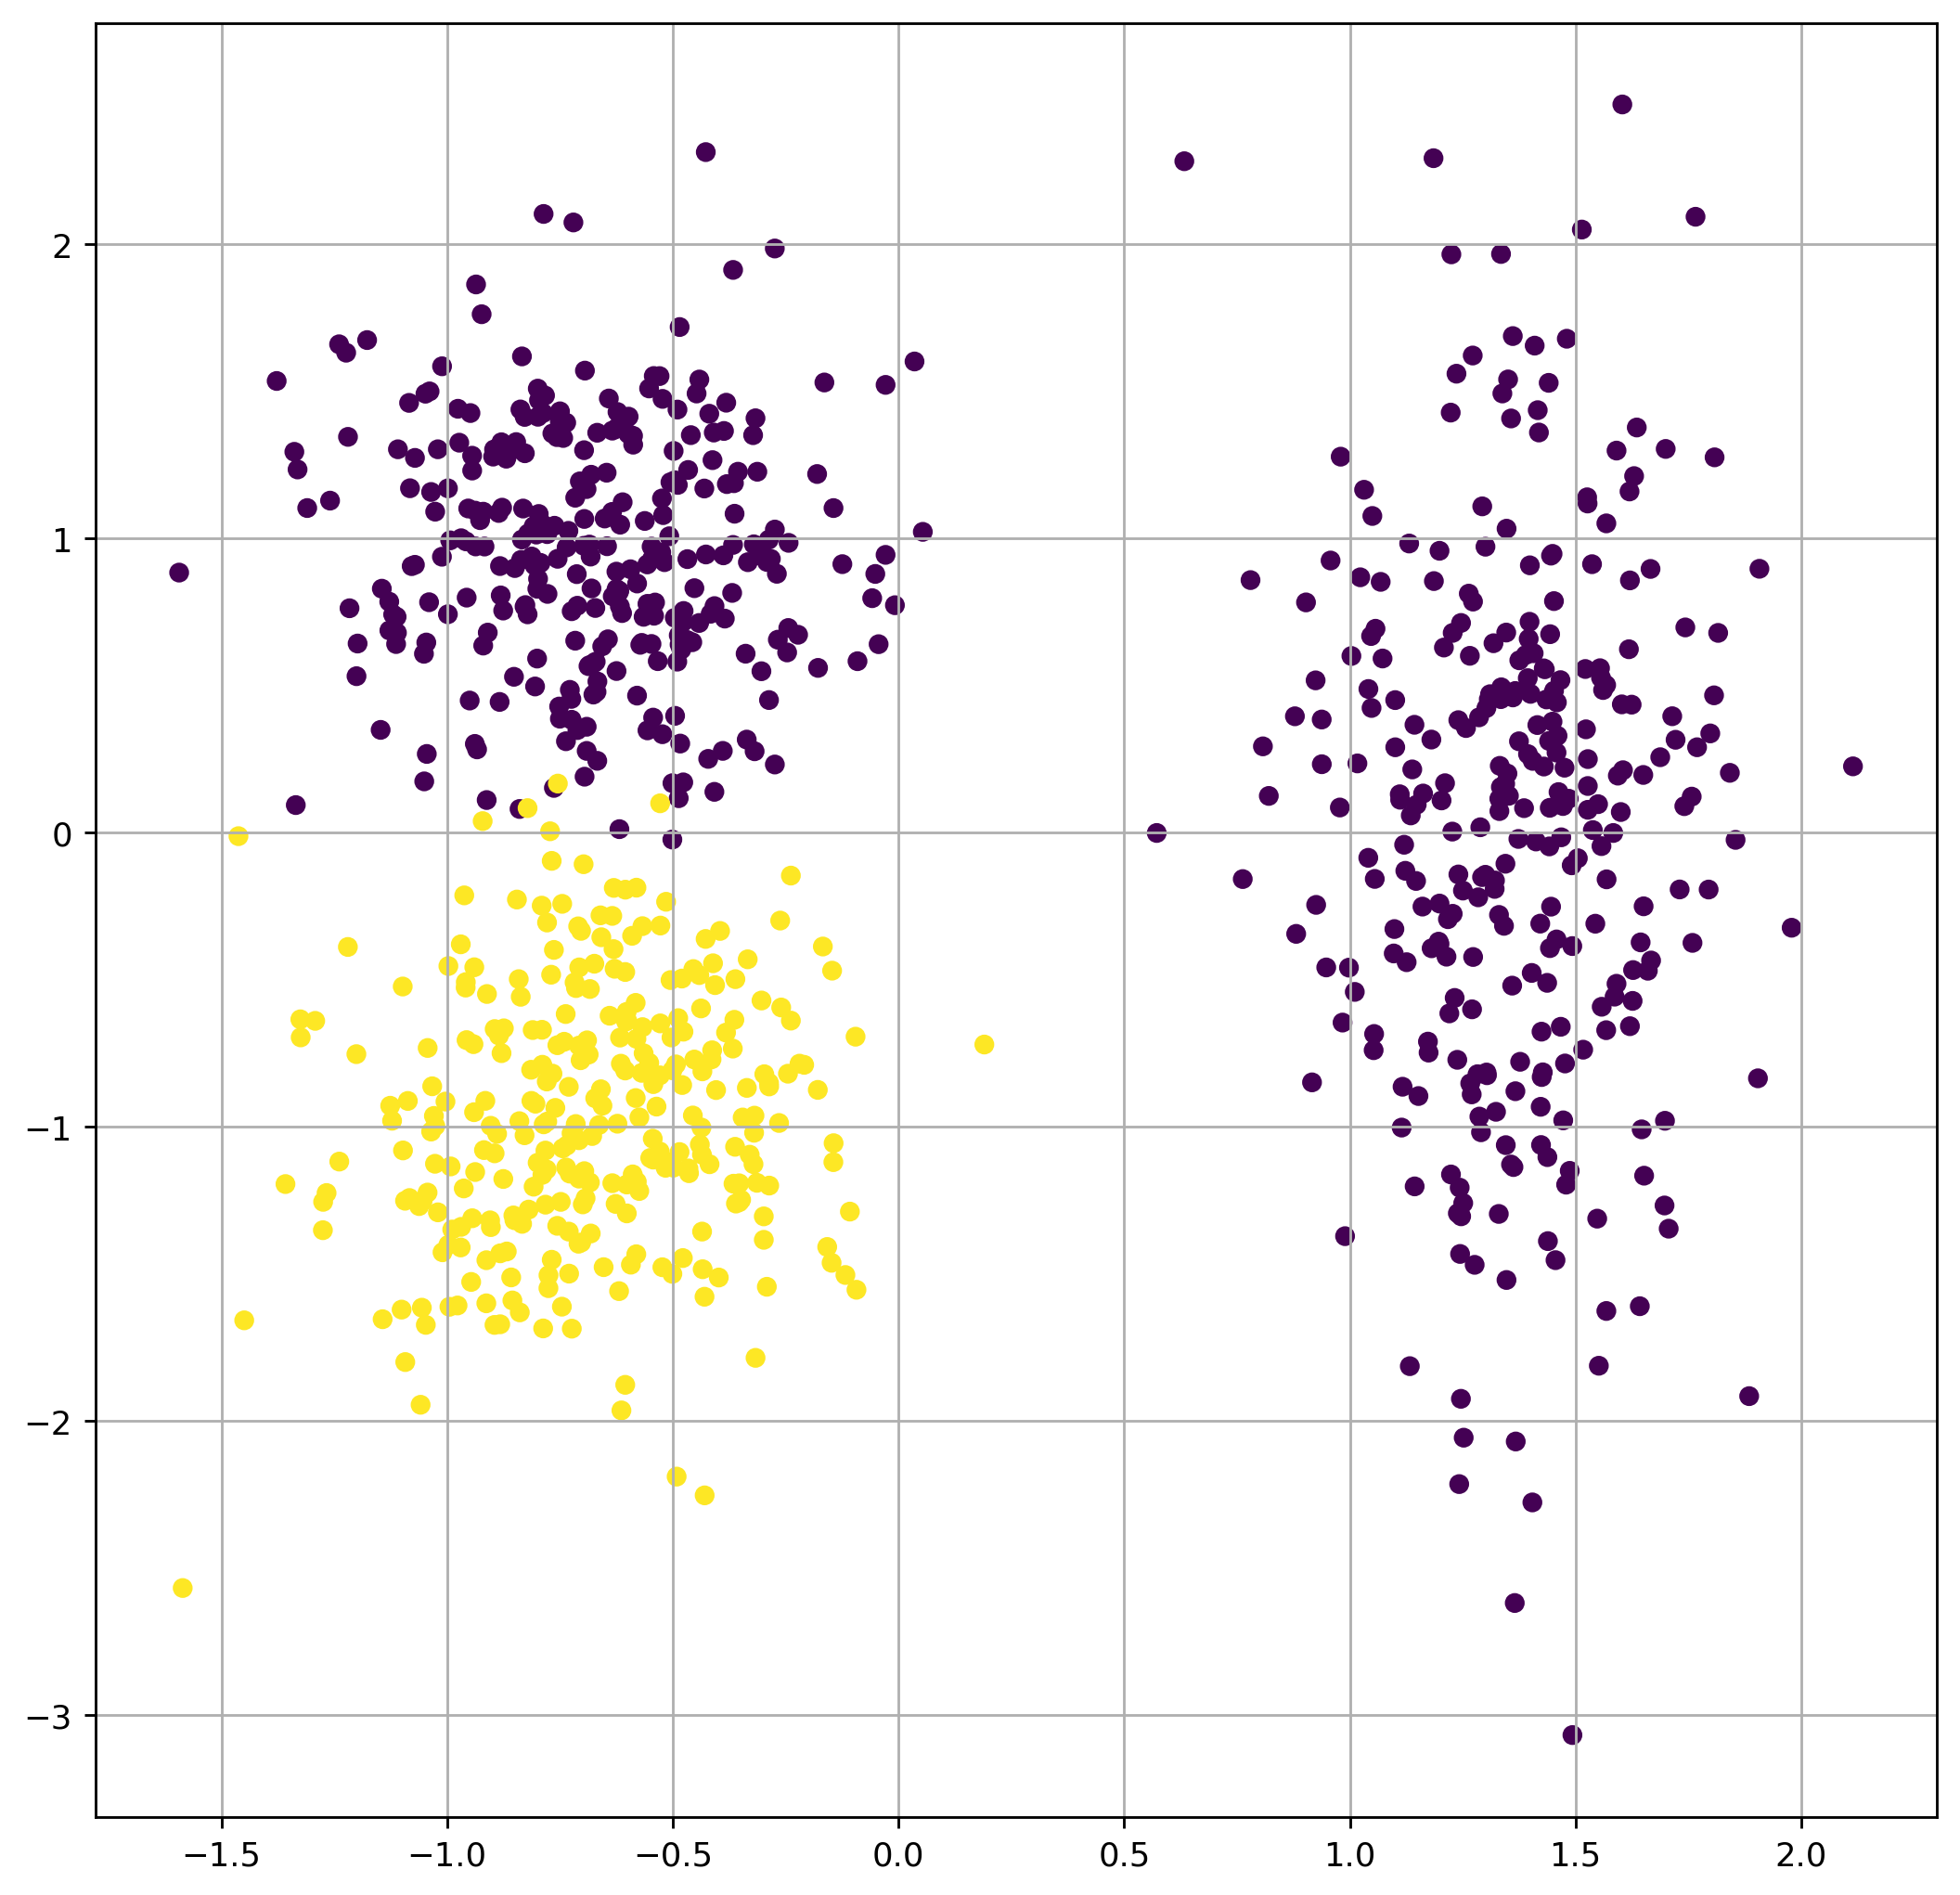
\includegraphics[width=.35\linewidth]{figures/example_groups/groups_centered}}
  ~
  \subfloat[\label{fig:ex-groups-after}]{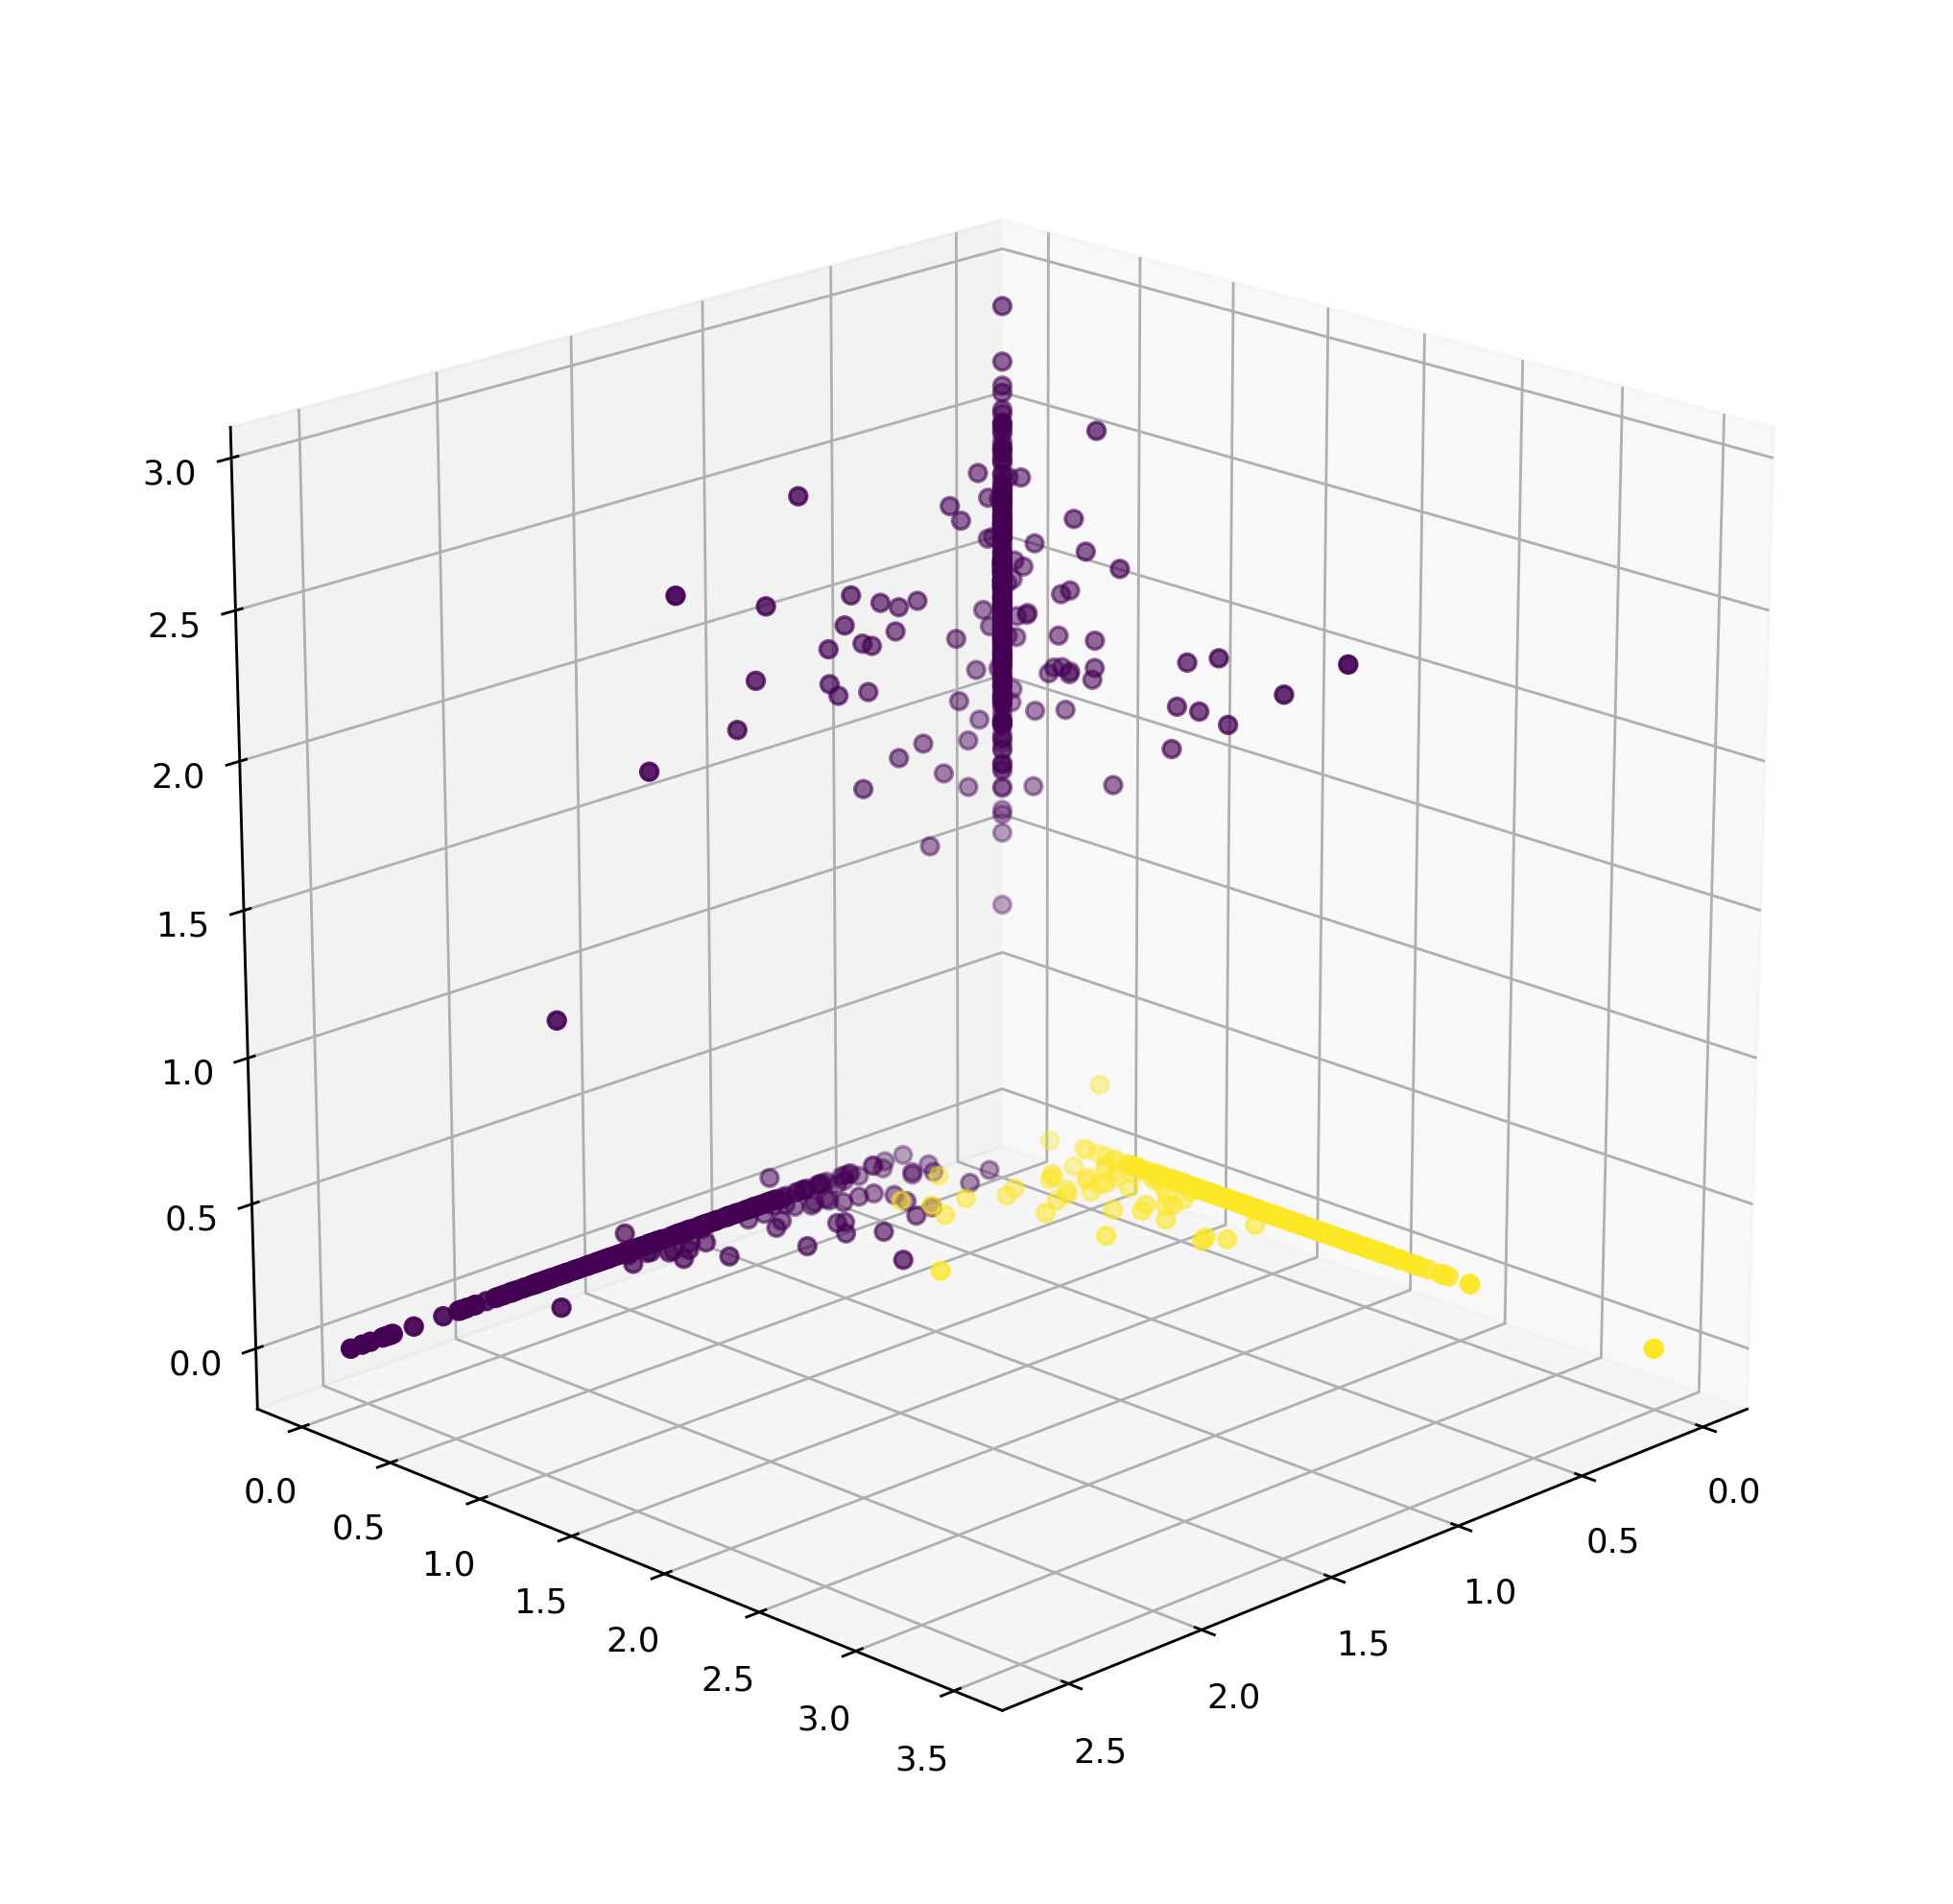
\includegraphics[width=.45\linewidth]{figures/example_groups/groups3d_centered}
  }
  \caption{(a) A 2D feature space with color-coded samples from two classes distributed in three groups. (b) After marker-based batch normalization and convolution with filters obtained from each group, the classes can be more easily detected by two filters in a new 3D feature space.}
  \label{fig:filter}
\end{figure}

Each convolutional layer is trained individually, one layer at a time, to find its filter set ${\cal F}$. The number of filters per layer depends on the clustering technique. We use $K$-means, and then the user must specify the number $K=|{\cal F}|$ of filters. After the convolution operation, we apply the ReLU function to eliminate negative activations and the max-pooling operation to aggregate local information. Note that, apart from the initial marker selection, the training process is automatic. We have preserved the convolutional layers' output dimensions and the marker pixels so we can find the filters of layer $L+1$ from the output of layer $L$. Figure~\ref{fig:arch} shows one example of a simple network projected by FLIM for the experiments of the next section. 

\begin{figure*}
  \begin{center}
  \tikzset{
    treenode/.style = {shape=rectangle, rounded corners,
                       draw=black, align=center, line width=width, minimum width=2cm},
    specialedge/.style = {line width=1.5pt}
  }

  \begin{tikzpicture}
    [
      grow                    = right,
      sibling distance        = 5em,
      level distance          = 30mm,
      edge from parent/.style = {draw=black, -latex},
      every node/.style       = {treenode},
      sloped
    ]
    \node [treenode, fill=tealDeer] {MarkerBased \\ BatchNorm}
    child {
        node [treenode, fill=tealDeer] {Conv$(60 \times 7 \times 7)$}
        child {
          node [treenode, fill=tealDeer] {ReLU} 
          child {
            node [treenode, fill=tealDeer] {MaxPool$(3\times3)$}
            child {
              node [treenode, fill=tealDeer] {BatchNorm}
              child {
                node [treenode, fill=navyPurple] {Classifier}
                edge from parent
              }
            }
          } 
        }
      };

  \end{tikzpicture}
  \end{center}
  \caption{Example of a network with a single convolutional layer followed by a classifier, as projected by FLIM and used for the experiments in this work.}
  \label{fig:arch}
\end{figure*}

\begin{figure*}
  \begin{center}
    
    \tikzstyle{steps} = [rectangle, rounded corners, minimum width=1.3cm, minimum height=0.5cm,text centered, draw=pink, thick, fill=heliotrope!30, execute at begin node={\begin{varwidth}{2.5cm}},
    execute at end node={\end{varwidth}}]
    \tikzstyle{image} = [minimum width=1.3cm, minimum height=0.7cm,text centered, draw=white,fill=white!30, inner sep=0pt]

    \tikzstyle{myarrow} = [navy, thick]

    \tikzstyle{arrow} = [thick,->,>=stealth]

    \begin{tikzpicture}[node distance=1.5cm]
    %images----------------------------
     \node (img1) [image] {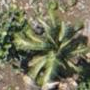
\includegraphics[width=.08\textwidth]{figures/qualitative/ours/lower-coco-789.png}};
     \node (img2) [image, below left=-5em of img1] {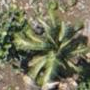
\includegraphics[width=.08\textwidth]{figures/qualitative/ours/lower-coco-789.png}};
     \node (img3) [image, below left=-5em of img2] {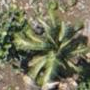
\includegraphics[width=.08\textwidth]{figures/qualitative/ours/lower-coco-789.png}};

     \node (imgs) [fit={($(img1.north west)+(-0.45,0.1)$) ($(img3.south east)+(0.45,-0.1)$)}, inner sep=0pt, draw=none, rounded corners, very thick, label = {[label distance = 0.1em]below:{Training set}}] {};
     %----------------------------------

     \node (tsne) [steps, right=1em of imgs] {t-SNE};

     \node (vis1) [image, right=1.5em of tsne, outer sep=0pt, label = {[label distance = 0.1em]below:{Projection}}] {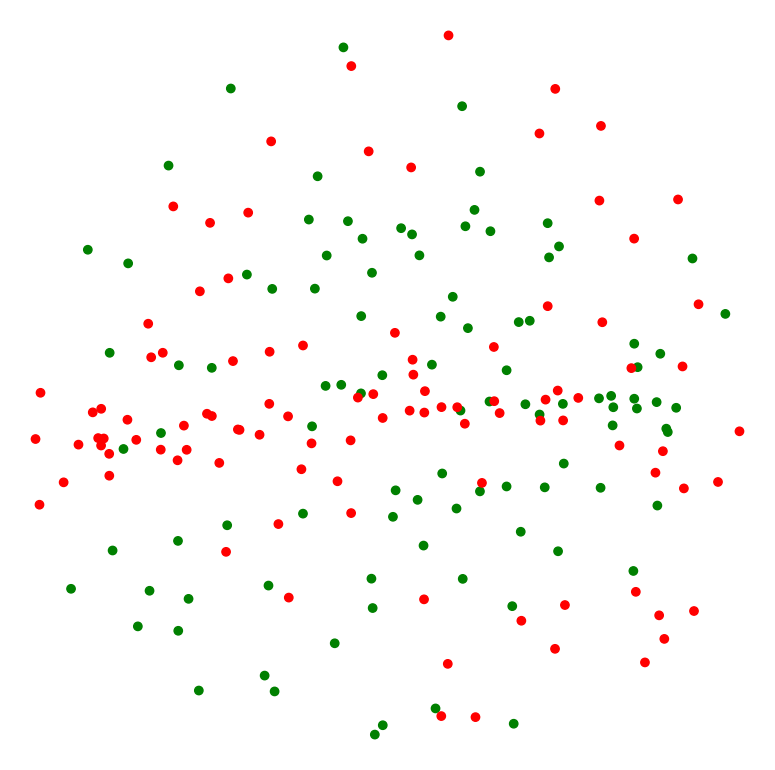
\includegraphics[width=.12\textwidth]{figures/input_200.png}};

     \node (select) [steps, right=1.35em of vis1] {Select\\ Images};
    
    %images----------------------------
    \node (simg1) [image, above right=-2.5em and 3em of select] {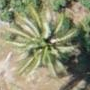
\includegraphics[width=.08\textwidth]{figures/img1.png}};
    \node (simg2) [image, below left=-5em of simg1] {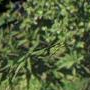
\includegraphics[width=.08\textwidth]{figures/img2.png}};
    \node (simg3) [image, below left=-5em of simg2] {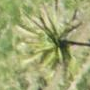
\includegraphics[width=.08\textwidth]{figures/img3.png}};
    \node (simg4) [image, below left=-5em of simg3] {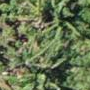
\includegraphics[width=.08\textwidth]{figures/img4.png}};

    \node (simgs) [fit={($(simg1.north west)+(-0.64,0.2)$) ($(simg4.south east)+(0.64,-0.2)$)}, inner sep=0pt, draw=none, label = {[label distance = 0.0em]above:{Selected images}}] {};
    %----------------------------------

     \node (put) [steps, right=1em of simgs] {Select\\Markers};

     %images----------------------------
    \node (mimg1) [image, above right=-2em and 2.8em of put] {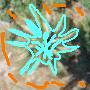
\includegraphics[width=.08\textwidth]{figures/markers1.png}};
    \node (mimg2) [image, below left=-5em of mimg1] {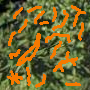
\includegraphics[width=.08\textwidth]{figures/markers2.png}};
    \node (mimg3) [image, below left=-5em of mimg2] {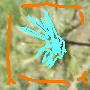
\includegraphics[width=.08\textwidth]{figures/markers3.png}};
    \node (mimg4) [image, below left=-5em of mimg3] {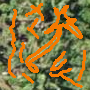
\includegraphics[width=.08\textwidth]{figures/markers4.png}};

    \node (mimgs) [fit={($(mimg1.north west)+(-0.64,0.2)$) ($(mimg4.south east)+(0.64,-0.2)$)}, inner sep=0pt, draw=none, label = {[label distance = 0.0em]above:{Markers}}] {};
    

    \node (flim) [steps, right=1em of mimgs] {FLIM};

    \node (ft) [steps, below=5em of flim] {Feature\\Extractor};


    \node (user) [image, below=2em of simgs, outer sep = -.5em] {
\includegraphics[width=.07\textwidth]{figures/user.png}};

     %--------------------------------------------------------------arrows
     \draw [arrow, myarrow] (imgs) -- (tsne);
     \draw [arrow, myarrow] (tsne) -- (vis1);
     \draw [arrow, myarrow] (vis1) -- (select);
     \draw [arrow, myarrow] (select) -- (simgs);
     \draw [arrow, myarrow] (simgs) -- (put);
     \draw [arrow, myarrow] (put) -- (mimgs);
     \draw [arrow, myarrow] (mimgs) -- (flim);
     \draw [arrow, myarrow] (flim) -- (ft);
     \draw [arrow, myarrow] (user) -- (select);
     \draw [arrow, myarrow] (user) -- (put);

     %\draw [decorate,decoration={brace,amplitude=10pt,raise=4pt},yshift=0pt]
%(img3.west) -- (img1.north) node [black,midway,xshift=0.8cm, label = {[label distance = 0.1em]above:{Images}}] {};

    \end{tikzpicture}
  \end{center}
  \caption{Pipeline to trian a feature extractor.}
  \label{fig:pipeline-xtractor}
\end{figure*}

  
\begin{figure*}
  \begin{center}
    
    \tikzstyle{steps} = [rectangle, rounded corners, minimum width=1.3cm, minimum height=0.5cm,text centered, draw=pink, thick, fill=heliotrope!30, execute at begin node={\begin{varwidth}{2.5cm}},
      execute at end node={\end{varwidth}}]
      \tikzstyle{image} = [minimum width=1.3cm, minimum height=0.7cm,text centered, draw=white,fill=white!30, inner sep=0pt]

    \tikzstyle{myarrow} = [navy, thick]

    \tikzstyle{arrow} = [thick,->,>=stealth]

    \begin{tikzpicture}[node distance=1.5cm]
      

      %images----------------------------
     \node (img1) [image] {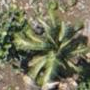
\includegraphics[width=.08\textwidth]{figures/qualitative/ours/lower-coco-789.png}};
     \node (img2) [image, below left=-5em of img1] {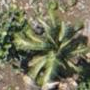
\includegraphics[width=.08\textwidth]{figures/qualitative/ours/lower-coco-789.png}};
     \node (img3) [image, below left=-5em of img2] {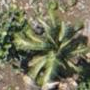
\includegraphics[width=.08\textwidth]{figures/qualitative/ours/lower-coco-789.png}};

     \node (imgs) [fit={($(img1.north west)+(-0.45,0.1)$) ($(img3.south east)+(0.45,-0.1)$)}, inner sep=0pt, draw=none, rounded corners, very thick, label = {[label distance = 0.1em]below:{Training set}}] {};
     %----------------------------------

     \node (aft) [steps, right=2em of imgs] {Apply Featute\\Extractor};

      %images----------------------------
    \node (f1) [image, above right=-3em and 3em of aft] {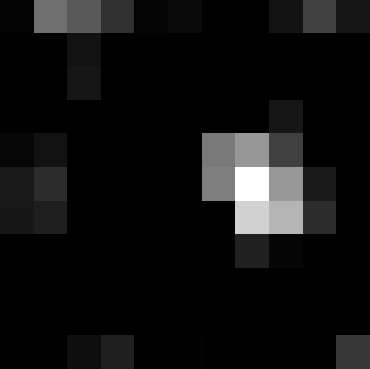
\includegraphics[width=.08\textwidth]{figures/features/f1.png}};
    \node (f2) [image, below left=-5.5em of f1] {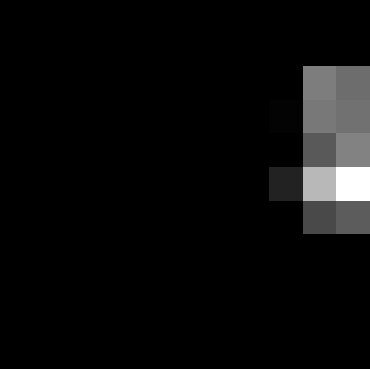
\includegraphics[width=.08\textwidth]{figures/features/f2.png}};
    \node (f3) [image, below left=-5.5em of f2] {
\includegraphics[width=.08\textwidth]{figures/features/f3.png}};
    \node (f4) [image, below left=-5.5em of f3] {
\includegraphics[width=.08\textwidth]{figures/features/f4.png}};

    \node (features) [fit={($(f1.north west)+(-0.3,0.2)$) ($(f4.south east)+(0.3,-0.2)$)}, draw=none, inner sep=0pt, label = {[label distance = 0.1em]below:{Features}}] {};
    %----------------------------------

     \node (sup) [steps, right=2em of features] {Supervised\\Learning};

     \node (clf) [steps, right=2em of sup] {Classifier};

     %--------------------------------------------------------------arrows
    
     \draw [arrow, myarrow] (imgs) -- (aft);
     \draw [arrow, myarrow] (aft) -- (features);
     \draw [arrow, myarrow] (features) -- (sup);
     \draw [arrow, myarrow] (sup) -- (clf);

    \end{tikzpicture}
  \end{center}
  \caption{Pipeline to train a classifier.}
  \label{fig:pipeline-classifier}
\end{figure*}

\section{Experiments}

We use a dataset from~\cite{8899005}, which contains regions of aerial images with and without coconut trees from the Kingdom of Tonga, as acquired in October 2017~\footnote{The images are available in \url{blog.werobotics.org/2018/01/11/open-ai-challenge-2}.}. Each region is classified as containing one or none coconut tree, but part of coconut trees from adjacent regions might appear near the region's border. The Humanitarian OpenStreetMap community annotated the regions. The dataset consists of 13587 regions with $90 \times 90$ pixels \textcolor{red}{with spatial resolution of $8$\si{\centi\metre}}, being 10268 and 3319 regions annotated as containing and not containing coconut trees, respectively. \textcolor{red}{The region images contain three channels: red, green, and blue. We convert them to the CIE L*a*b* color space and normalize each channel within $[0,1]$}.





To assess the impact of FLIM in reducing the need for annotated samples, we
divided the experiments in three parts. First, we randomly selected 200 regions (100 from each class) for training, 1000 regions (500 from each class) for the choice of architecture, and left the remaining 12387 regions for testing. The architecture of the network was chosen based on empirical tests on the validation set. Second, we used the validation set to increase the size of the training set from 200 to 1200 images. 

\textcolor{red}{We repeated this procedure three times to compute the mean and the standard deviation of the results in precision, recall, and f-score.} By vectorizing and projecting the 200 training images of each split on 2D with t-SNE~\cite{maaten2008visualizing}, \textcolor{red}{we identified cohesive groups of images from each class and selected two representative images from each class to draw markers.}  The selected images from one split can be seen in Figure \ref{fig:markers}. We placed markers on these images in regions that we thought to better distinguish between coconut and non-coconut classes.

\textcolor{red}{We have not investigated the impact of placing markers on a higher number of images and network architecture optimization procedures yet.} We just trained the single-convolutional-layer network of Figure \ref{fig:arch} from markers drawn in two images per class. The convolutional layer has $60$ filters with dimension $7 \times 7$ and 3 color channels. It includes marker-based normalization before convolution, ReLu activation, and a max-pooling operation with a window of dimension $3 \times 3$. Since it is the single and last convolutional layer, we applied a stride of $4$ in max-pooling and batch normalization to create an input as close as possible to the one of the \textcolor{red}{MLP} classifier used in the popular VGG-16~\cite{simonyan2014very}. \textcolor{red}{We use Pytorch to implement our feature extractor and the MLP classifier.The experiments used an Intel(R) Xeon(R) CPU E5-2620 v4 @ 2.10GHz CPU and a Titan X with 12 GB of memory.} We trained the MLP classifier for $40$ epochs and the whole network for $60$ epochs with a batch size of $64$. We use a learning rate of $0.0001$, a weight decay of $0.001$, and we update the learning rate by a factor of $0.1$ every $5$ epochs after epoch 30.

We selected VGG-16 for comparative analysis since it usually requires many more samples than 200 to be trained from scratch. It is also a very competitive CNN when pretrained in the ImageNet dataset, working as a counterpart solution for small training sets. Therefore, as baselines, we used three solutions based on VGG-16: (1) VGG is trained from scratch, (2) VGG-FT is pretrained in the ImageNet dataset and fine-tuned in the coconut-tree training set, and (3) VGG-FE is the feature extractor of VGG-16 (the output of its last convolutional layer) pretrained in the ImageNet dataset. In this case, we used for classification the  linear SVM classifier with $C=0.01$ from sklearn~\cite{fan2008liblinear, scikit-learn}. We use Pytorch's implementation of VGG. In (1) and (2), we trained for $95$ epochs with a batch size of $64$, learning rate of $0.001$, weight decay of $0.001$, and we update learning rate by a factor of $0.1$ every $5$ epochs after the model achieves an accuracy of $0.95$.

Table~\ref{tab:results} shows the results of three FLIM-based solutions using the SVM and MLP classifiers; ``FLIM+SVM'', ``FLIM+MLP'', and ``FLIM-FT+MLP'' (i.e., FLIM with fine-tuning); as compared with the VGG-based solutions above. The first two rows indicate that FLIM  can provide a more effective feature extractor using a single convolutional layer than VGG-FE, which contains 13 convolutional layers pretrained on the ImageNet. The results of ``FLIM+MLP'' and ``FLIM-FT+MLP'' show that FLIM  may dismiss fine tuning by directly providing a more effective solution. \textcolor{red}{By comparing ``FLIM+MLP'' with VGG, one can observe that FLIM reduces the number of required training images.} Finally, the comparison between \textcolor{red}{``FLIM+MLP'' and VGG-FT} demonstrates that FLIM can provide competitive results using a considerably more simplified architecture than  VGG-FT. The number of parameters of our feature extractor represents only $0.07\%$ of the number of parameter of VGG-FE.

\begin{figure}[!t]
    \centering
    \subfloat[\label{fig:markers1}]{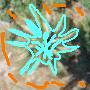
\includegraphics[width=.25\linewidth]{figures/markers1}
    }
    ~
    \subfloat[\label{fig:markers2}]{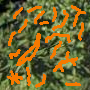
\includegraphics[width=.25\linewidth]{figures/markers2}
    }
    \\
    \subfloat[\label{fig:markers3}]{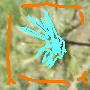
\includegraphics[width=.25\linewidth]{figures/markers3}
    }
    ~
    \subfloat[\label{fig:markers4}]{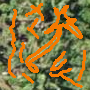
\includegraphics[width=.25\linewidth]{figures/markers4}
    }
    \caption{\textcolor{red}{Markers used for training in image regions with (first column) and without (second column) a coconut tree.}}
    \label{fig:markers}
\end{figure}

\begin{table}[!t]
  \begin{center}
  \begin{tabular}{|l|c|c|c|}
  \hline
   Method & Precision & Recall & F-score \\
  \hline\hline
    FLIM+SVM & $0.856 \pm 0.011 $ & $ 0.831 \pm 0.019$ & $ 0.838 \pm 0.017$\\ 
    VGG-FE+SVM & $0.855 \pm 0.001$ & $0.816 \pm 0.007$ & $0.826 \pm 0.006 $ \\\hline
      
    FLIM+MLP & $0.863 \pm 0.002$ & $0.849 \pm 0.005$ & $0.854 \pm 0.004$\\
    FLIM-FT+MLP & $0.845 \pm 0.003$ & $0.825\pm 0.006$ & $0.832 \pm 0.005$ \\

    VGG & $0.827 \pm 0.003$ & $0.770 \pm 0.016$  & $ 0.784 \pm 0.014$\\
    VGG-FT & $0.872 \pm 0.007$ & $0.844 \pm 0.015$ & $0.851 \pm 0.014 $ \\
   
  \hline
  \end{tabular}
  \end{center}

\caption{Mean and standard deviation of precision, recall, and f-score for each method: a feature extractor with a classifier.}
  \label{tab:results}
\end{table}



\begin{figure}
  \centering
  \subfloat{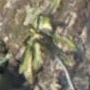
\includegraphics[width=.2\linewidth]{figures/qualitative/ours/upper-coco-108.png}
  }
  ~
  \subfloat{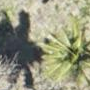
\includegraphics[width=.2\linewidth]{figures/qualitative/ours/upper-coco-2473.png}
  }
  ~
  \subfloat{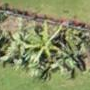
\includegraphics[width=.2\linewidth]{figures/qualitative/ours/upper-non_coco-506.png}
  }
  \\
  \subfloat{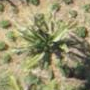
\includegraphics[width=.2\linewidth]{figures/qualitative/vgg/lower-coco-1098.png}
  }
  ~
  \subfloat{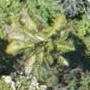
\includegraphics[width=.2\linewidth]{figures/qualitative/vgg/lower-coco-875.png}
  }
  ~
  \subfloat{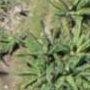
\includegraphics[width=.2\linewidth]{figures/qualitative/vgg/lower-non_coco-105.png}
  }
  \caption{Misclassified images by ``FLIM + MLP'' (first row) and VGG-FT (second row), being the last column with images without coconut trees.}
  \label{fig:ex-classification}
\end{figure}

 In Figure \ref{fig:ex-classification}, we can see examples of misclassified images. In these images, coconut trees appear in different angles, sizes, and shapes, or the boundaries between the coconut tree and the background are tenuous, making it more difficult to identify them. In turn, images that do not contain coconut trees, contain trees that resemble their shape. The network designer could add markers in those images to improve the feature extractor in an active learning loop.

\begin{figure}
  \centering
  \subfloat[\label{fig:vis-input}]{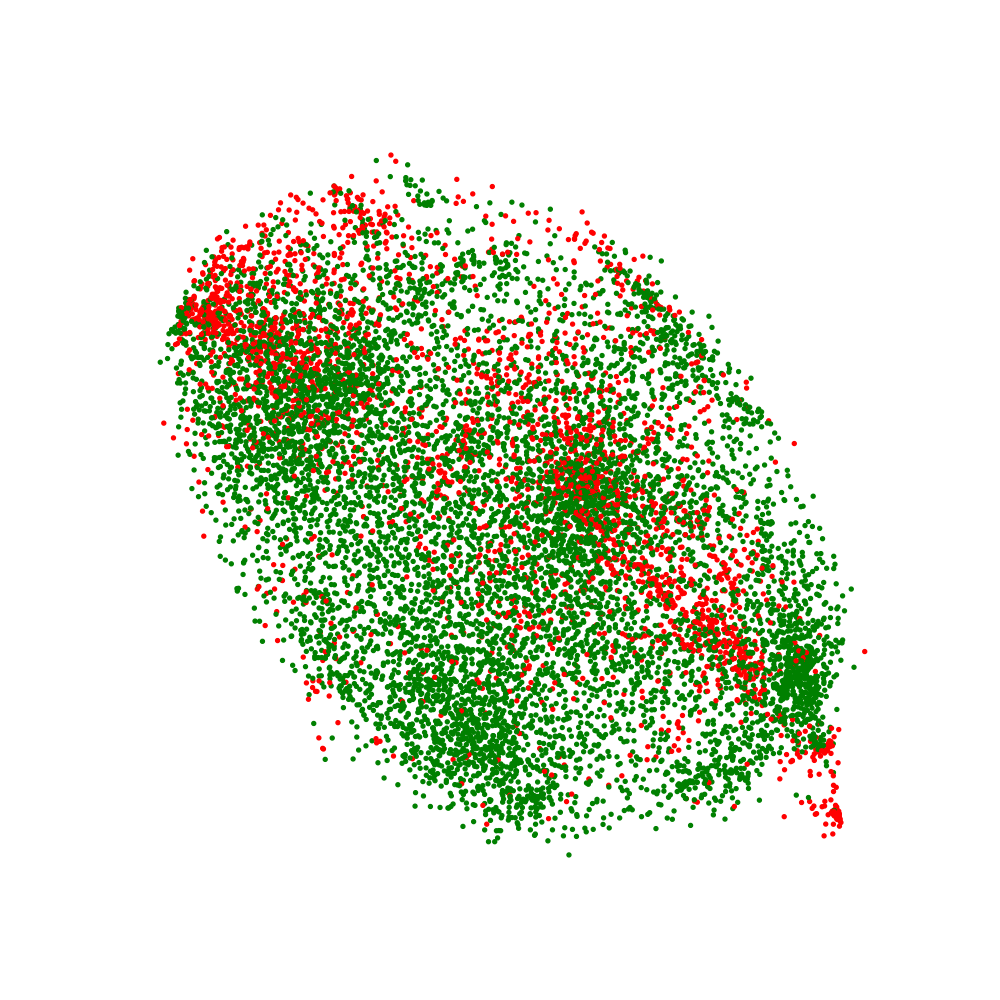
\includegraphics[width=.3\linewidth]{figures/input}
  }
  ~
  \subfloat[\label{fig:vis-feature-extractor}]{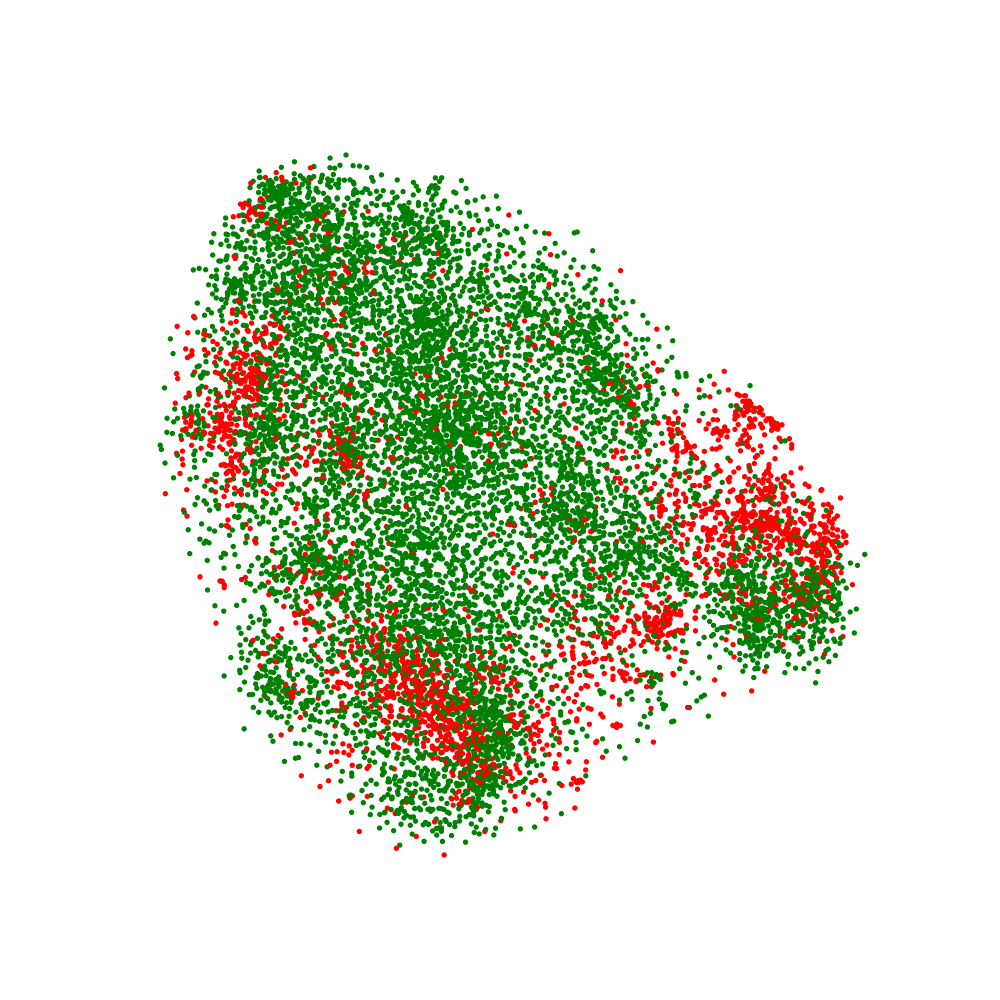
\includegraphics[width=.3\linewidth]{figures/feature_extractor}
  }
  ~
  \subfloat[]{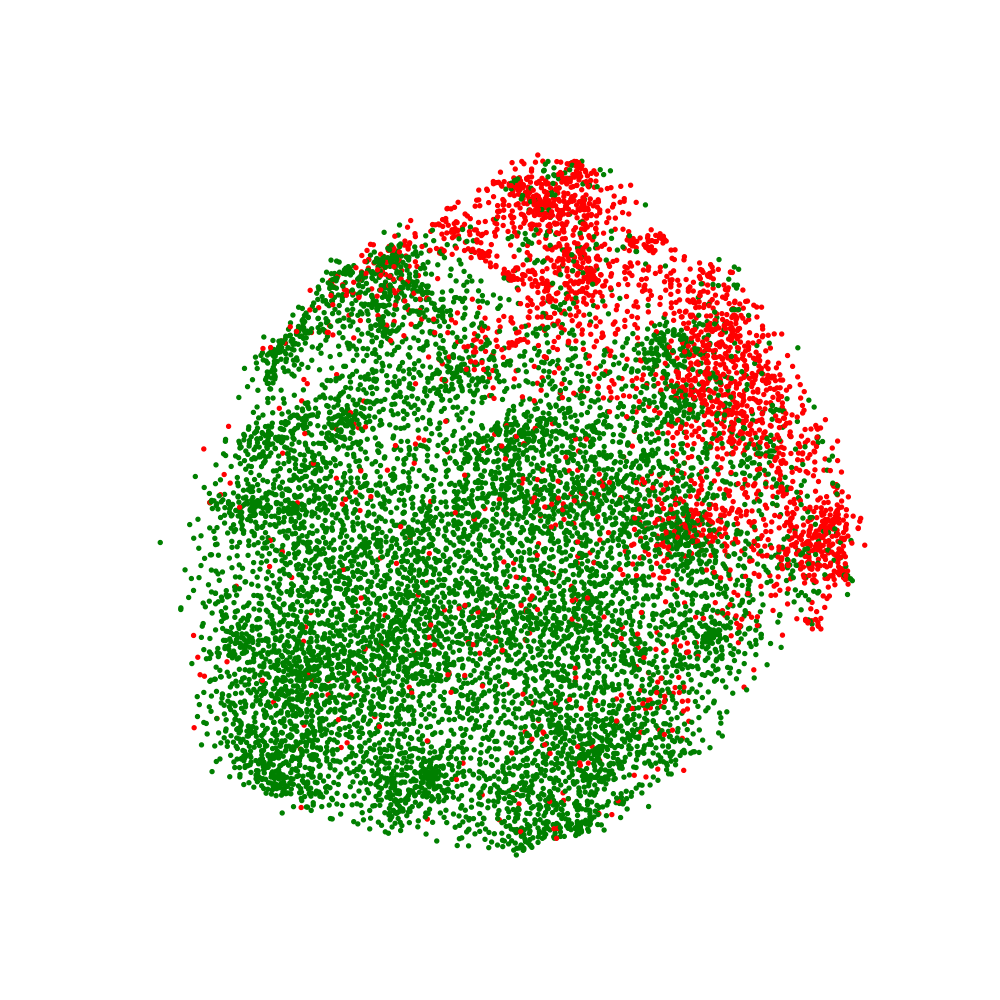
\includegraphics[width=.3\linewidth]{figures/classifier}
  \label{fig:vis-classifier}}
  \caption{Projections by t-SNE of the test images at (a) the input layer, (b) the output of the convolutional layer of  ``FLIM + MLP'' after batch normalization (Figure~\ref{fig:arch}), and (c) the output of the last hidden layer of the MLP classifier in  ``FLIM + MLP''.}
\end{figure}

As motivated by Rauber et al. \cite{rauber2016visualizing}, we created projections of three stages of the network ``FLIM + MLP" using t-SNE \cite{maaten2008visualizing} to understand how our CNN transforms image spaces along its layers. In Figure \ref{fig:vis-input}, we can see the projection of the test images in the LAB color space. Green points are images that contain coconut trees, and red points are images that do not contain coconut trees. The projection shows considerable overlapping between the two classes. The samples of both classes are also dispersed in the projection. In Figure \ref{fig:vis-feature-extractor}, the projection of the output of our feature extractor shows some reduction in sample dispersion. The classes show more concentration in some parts of the projection and reduced overlapping between them. Finally, Figure \ref{fig:vis-classifier} shows the output of the last hidden layer of the MLP classifier in ``FLIM + MLP''. The overlapping between classes and sample dispersion are considerably reduced, explaining our results.

\begin{comment}
  \begin{table}[!t]
  \begin{center}
  \begin{tabular}{|l|c|c|c|}
  \hline
   Method & Precision & Recall & F-score \\
  \hline\hline
    FLIM+MLP & $0.894 \pm 0.006$ & $0.888 \pm 0.009$ & $0.890 \pm 0.008$\\
    FLIM-FT+MLP & $0.888 \pm 0.001$ & $0.878\pm 0.001$ & $0.881 \pm 0.001$ \\
    VGG-FT & $0.884 \pm 0.003$ & $0.877 \pm 0.006$ & $0.879 \pm 0.005 $ \\
  \hline
  \end{tabular}
  \end{center}
  \caption{Mean and standard deviation of precision, recall, and f-score for each method: a feature extractor with a classifier with a larger train set.}
    \label{tab:results-with-1200-images}
  \end{table}
\end{comment}



\begin{figure}
\begin{tikzpicture}
  \begin{axis}[
    /pgf/number format/set thousands separator = {},
    xlabel = Training set size,
    ylabel = f-score,
    xmin=300, xmax=1200,
    grid=major,
    grid style=dashed,
    xtick={300,450, 600, 750, 900, 1050, 1200},
    legend style={nodes={scale=0.65, transform shape}},
    legend pos=south east
    ]
    \addplot table[x index=0,y index=1,header=false] {data/data.dat};
    \addlegendentry{FLIM+MLP}

    \addplot  table[x index=0,y index=2,header=false] {data/data.dat};
    \addlegendentry{FLIM-FT+MLP}

    \addplot  table[x index=0,y index=3,header=false] {data/data.dat};
    \addlegendentry{VGG-FT}

    \addplot table[x index=0,y index=4,header=false] {data/data.dat};
    \addlegendentry{CL+MLP}

    \legend{FLIM+MLP,FLIM-FT+MLP,VGG-FT,CL+MLP}
  
  \end{axis}
\end{tikzpicture}
\caption{Graph showing the impact of training set size on quantitative results. FLIM+MLP feature extractor was trained only with four images, and the remaining training set was used to train the MLP classifier.}
\end{figure}

\section{Conclusion}

We introduced a first feature learning technique, named FLIM, that can estimate effective filter weights for the convolutional layers of a given network architecture from user-drawn markers in a few training images. The resulting feature extractor can be used with different classifiers and, when it is used with a MLP classifier, the number of required images to train the fully connected layers is reduced. We demonstrated the advantages of FLIM over solutions based on VGG-16 for the binary classification of coconut-tree images. The experiments indicated that FLIM is an effective approach to produce considerably simplified network architectures. By involving the user in the training process, FLIM improves the understanding about CNN models and the user control over the training process. 

We intend to further investigate feature learning from image markers for different applications, elaborate methodologies to optimize network architecture, and extend FLIM to estimate weights in fully connected layers.   

\section*{Acknowledgements}

This research was funded by FAPESP (2014/12236-1), CNPq (303808/2018-7), Petróleo Brasileiro S.A. (PETROBRAS) and Agência Nacional do Petróleo, Gás Natural e Biocombustíveis (ANP), Grant Numbers 4600556376 and 4600583791.
\bibliographystyle{IEEEtran}
\bibliography{bibliography}

\end{document}


